\documentclass[a4paper, 12pt]{article}

\usepackage[protrusion=true,expansion=true]{microtype} % Better typography
\usepackage{graphicx} 
\usepackage{subfig}
\usepackage{wrapfig} %in-line image

\usepackage[dvipsnames]{xcolor}
\usepackage{listings}
\usepackage[italian]{babel}
\usepackage[T1]{fontenc} 
\usepackage[utf8]{inputenc}

\usepackage[hyphens]{url}
\usepackage{quoting}
%\usepackage[unicode,pdftex,plainpages=false,linktoc=all, hyperindex,citecolor=green,urlcolor=blue ]{hyperref}
\quotingsetup{font=small}

\usepackage[%printonlyused
]{acronym}

\makeatletter
\newcommand{\myparagraph}[1]{\paragraph{#1}\mbox{}\\}
\renewcommand\@biblabel[1]{\textbf{#1.}} % Change the square brackets for each bibliography item from '[1]' to '1.'
\renewcommand{\@listI}{\itemsep=0pt} % Reduce the space between items in the itemize and enumerate environments and the bibliography

% \renewcommand{\abstractname}{\large Introduction} %%Renaming the abstract

%-----title at right corner---------------------------------------
\renewcommand{\maketitle}{ 
\begin{figure}[h]
\centering

\includegraphics[width=7cm]{Images/LogoPolimi}\\[.5cm]
\end{figure}

\vspace{50pt}

\begin{flushright} % Right align
\@date 

{\huge\@title} % Increase the font size of the title
\vspace{140pt} % Some vertical space between the title and author name


\begin{tabular}{ l l c}
\large Blanco &  \large Federica & \large 875487\\
\large Pennati & \large Giulia & \large 882962\\
\end{tabular}

\vspace{40pt} % Some vertical space between the author block and abstract
\end{flushright}
\centering
\textsl{\large Advanced User Interface Project}\\
2017/2018
}


\title{\textbf{GEA}\\[3mm]
Gioco Educazione Alimentare}

\author{Blanco Federica\\Pennati Giulia%\textsc{Nomi} % Author -> fix with more names
} 

\date{INSERIREMO DATA CONSEGNA} % Date

%----------------------------------------------------------------------------------------

\begin{document}

\begin{titlepage}

\thispagestyle{empty}
\maketitle % Print the title section

\end{titlepage}


%\input{Acronym.tex}
%\renewcommand{\abstractname}{Summary} % Uncomment to change the name of the abstract to something else
%\vspace{30pt} % Some vertical space between the abstract and first section
\thispagestyle{empty}
\tableofcontents
\clearpage 
\thispagestyle{empty}
\listoffigures
\clearpage 
%\listoftables
%\clearpage 

\newpage
\pagenumbering{arabic}
\section{Introduzione} \label{sec:intro}
Il termine disturbo neurologico, \acs{ndd}, racchiude al suo interno tutte le condizioni che sono causate da una disfunzione di una parte del cervello o del sistema nervoso che mostrano alcuni sintomi nello sviluppo fisico e psicologico del bambino \cite{rif1}. Tra le malattie più comuni troviamo l'Autismo, \acs{asd}, il deficit dell'attenzione e iperattività, \acs{adhd}, e la sindrome di Down \cite{rif2}. I bambini che soffrono di queste sindromi hanno bisogno di un aiuto nello sviluppo di abilità cognitive quali attenzione e linguaggio, abilità sociali quali la capacità di relazionarsi con gli altri e abilità di autonomia personale e domestica. I grandi benefici dell'utilizzo della Realtà Virtuale in un contesto educativo e riabilitativo sono ormai riconosciuti a livello mondiale e provati tramite vari test comparativi tra riabilitazione con l'uso di nuove tecnologie e riabilitazione con l'uso di metodi classici \cite{rif3}, \cite{rif4}, \cite{rif5}. Il nostro progetto si focalizza proprio su questo aspetto e sulla propensione dei bambini nel voler avere un'esperienza con strumentazioni quali visori \acs{vr} perchè risultano affascinanti e attrattivi, nonostante un po' di titubanza per possibile sensazione di nausea. \acs{gea}, \acl{gea}, si pone come obiettivo quello di aiutare grazie all'uso della \acs{vr} i bambini a sviluppare una autonomia propria e domestica nel campo dell'alimentazione, di grandissima importanza al giorno d'oggi come dimostrato durante il recente Expo tenutosi a Milano. Grazie a questo gioco i bambini alleneranno la memoria per ricordare i vari livelli della piramide alimentare, impareranno a riconoscere i cibi sani da quelli cosiddetti "spazzatura" e capiranno come abbinare un pasto della giornata ad una pietanza e viceversa. \acs{gea} viene sviluppata come app per smartphone ma con la necessaria replicazione dello schermo sul computer della terapista in modo che possa seguire tutto quello che il bambino compie durante l'esperienza di gioco. Nelle sezioni successive saranno spiegati in maggiore dettaglio lo stato dell'arte, i requisiti e bisogni dei nostri stakeholder, le tecnologie hardware e software utilizzate per lo sviluppo e gli scenari rappresentativi.
\newpage
\section{Stato dell'Arte} \label{sec:stato}
\newpage
\section{Bisogni e Requisiti} \label{sec:biso}
The problem that you want to address
o Main Target Groups
o Context and Needs addressed
o (Constraints)
o Goals of your project

\subsection{Target Group} \label{subsec:target}
\acs{gea} è rivolto ai bambini affetti da \acs{ndd} ossia da malattie neurologiche, in particolare i nostri principali utenti sono seguiti da terapisti che li aiutano nel loro percorso e portano avanti un progetto di educazione alimentare che si svolge durante un laboratorio con personale qualificato.

\subsection{Stakeholder e Bisogni} \label{subsec:stakbis}
I nostri stakeholder sono divisi essenzialmente in tre categorie:
\begin{itemize}
\item Utenti primari (end user): bambini affetti da sindrome \acs{ndd}
\item Utenti secondari: terapisti
\item Utenti terziari: familiari, sviluppatori, manager
\end{itemize}
Il bisogno che la nostra applicazione cerca di soddisfare è un necessario sviluppo di un'autonomia personale e domestica nel campo dell'alimentazione: aumentare dunque la capacità di stabilire in autonomia quali cibi è corretto mangiare, in quante dosi e a quali pasti del giorno.


\subsection{Obiettivo del progetto} \label{subsec:obiettivo}
L'obiettivo del progetto \acs{gea} è creare un'applicazione in grado di insegnare ai bambini affetti da \acs{ndd} l'educazione alimentare tramite un'esperienza di gioco interattiva.


\subsection{Contesto} \label{subsec:contesto}
Il contesto di utilizzo di \acs{gea} è una stanza in un centro specializzato durante una seduta di laboratorio di alimentazione con la presenza di una terapista.


\subsection{Vincoli} \label{subsec:vincoli}
Vi sono svariati vincoli da dover rispettare:
\begin{itemize}
\item Basso costo
\item Grande facilità di utilizzo
\item Basso consumo di energia
\item Connessione internet attiva
\item Limitazioni sulla grafica: evitare colori freddi o alcuni tipi di animazioni
\item Necessità di spiegazioni visive in quanto alcuni utenti non sanno leggere
\end{itemize}


\subsection{Requisiti iniziali} \label{subsec:requis}
Per quanto riguarda i dispositivi necessitiamo di:
\begin{enumerate}
\item Smartphone con applicazione \acs{gea} installata
\item Visore di realtà virtuale
\item Pc
\item Google Chromecast
\end{enumerate}

Per quanto riguarda l'interazione con l'applicazione essa avverrà con due modalità differenti: ci sarà un'interazione di tipo touchscreen all'avvio di \acs{gea} per permettere alla terapeuta di scegliere il gioco da far svolgere al ragazzo e con quale difficoltà, l'interazione diventa poi di tipo visivo per la partita vera e propria in quanto le varie risposte verranno date con il movimento oculare.


\acs{gea} è un gioco con diverse funzionalità quali l'esercizio della memoria, abilità di problem solving, capacità di decision making e learning tool.


\newpage
\section{UXDesign} \label{sec:design}

\subsection{Approccio generale} \label{subsec:app}
In questa sezione mostriamo i diagrammi di flusso rappresentativi dell'intera applicazione e dei singoli giochi.

La Figura \ref{fig:Diagramma di flusso generale} mostra il diagramma di flusso dell'intera applicazione: all'avvio dell'applicazione si hanno in sequenza la scelta del gioco, la scelta del livello di difficoltà e poi l'avvio della partita composta da tre sessioni di gioco. Al termine delle tre sessioni la partita viene chiusa mostrando il punteggio totalizzato.

La Figura \ref{fig:Diagramma di flusso del gioco "Impara con la piramide} mostra il diagramma di flusso del gioco "Impara con la piramide": in sequenza si hanno la visualizzazione dell'intera piramide incompleta e lo zoom sullo specifico livello da completare con l'apparizione delle due opzioni tra cui scegliere. Nel caso di scelta corretta verrà mostrato il feedback corrispondente e incrementato il punteggio, nel caso di scelta erronea verrà solamente mostrato il feedback.

La Figura \ref{fig:Diagramma di flusso dei giochi "E' sano o no?" e "A tavola!"} mostra il diagramma di flusso dei giochi "E' sano o no?" e "A tavola!". Per entrambi verrà mostrata la schermata iniziale con le opzioni tra cui scegliere: nel caso di scelta corretta verrà mostrato il feedback corrispondente e incrementato il punteggio, nel caso di scelta erronea verrà solamente mostrato il feedback.

\begin{figure}[htbp]
\centering
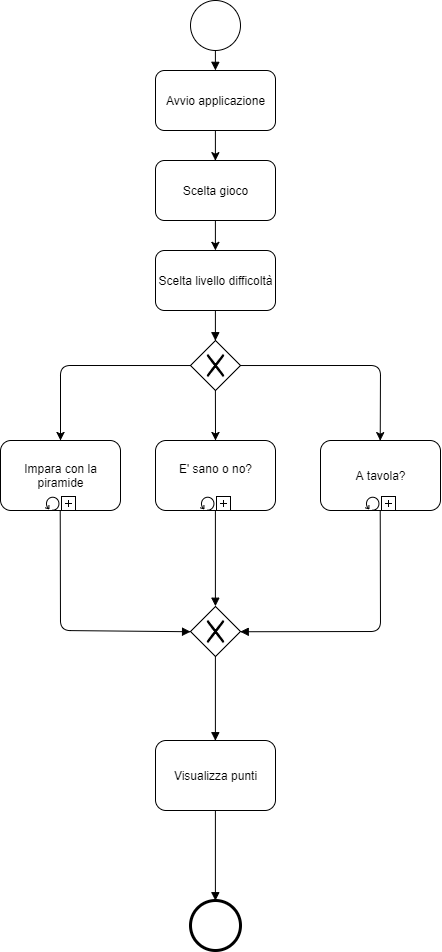
\includegraphics[scale=0.6]{Images/Flussogenerico}
\caption{Diagramma di flusso generale}
\label{fig:Diagramma di flusso generale}
\end{figure}
\clearpage

\begin{figure}[htbp]
\centering
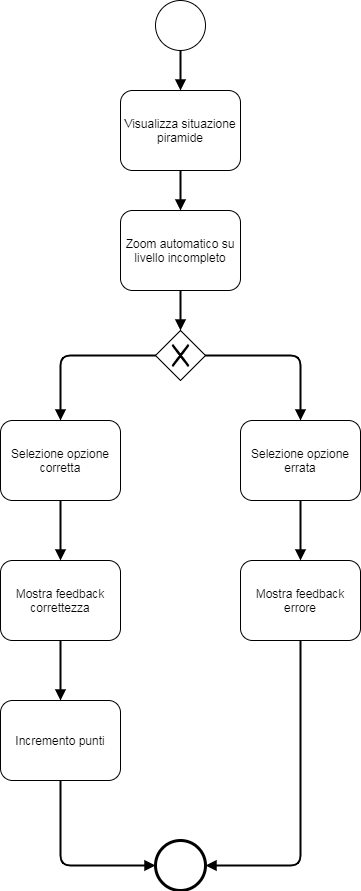
\includegraphics[scale=0.6]{Images/Flussopiramide}
\caption{Diagramma di flusso del gioco "Impara con la piramide"}
\label{fig:Diagramma di flusso del gioco "Impara con la piramide}
\end{figure}
\clearpage

\begin{figure}[htbp]
\centering
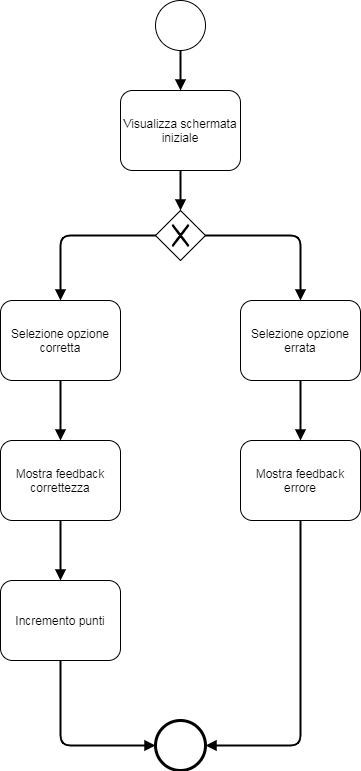
\includegraphics[scale=0.7]{Images/Flusso23}
\caption{Diagramma di flusso dei giochi "E' sano o no?" e "A tavola!"}
\label{fig:Diagramma di flusso dei giochi "E' sano o no?" e "A tavola!"}
\end{figure}
\clearpage

\subsection{Scenari} \label{scenari}
Di seguito vengono riportati tre scenari a rappresentazione dei giochi che si possono fare con \acs{gea}, sono tutti e tre di tipo testuale.
\subsubsection{Scenario 1}
Maria, terapista di un centro terapeutico per persone con disabilità, si trova nel suo studio pronta ad accogliere Emanuele, bimbo affetto da \acs{ndd}, per proseguire il loro percorso di educazione alimentare. Durante questa fase del laboratorio Maria decide di far uso di \acs{gea}, gioco di realtà virtuale per l'educazione alimentare, partendo da un livello basso di difficoltà. All'arrivo del bambino essa dunque avvia l'applicazione sopracitata e grazie al touchscreen seleziona il gioco "Impara con la piramide" perchè ha notato che Emanuela ha difficoltà nell'imparare quali alimenti si trovano in ogni specifico livello della piramide alimentare. Seleziona poi il livello "Facile" tra quelli possibili presentati e inserisce lo smartphone nel visore che il bambino va ad indossare. Il gioco mostra ad Emanuele prima l'intera piramide incompleta, poi si va a focalizzare su uno specifico livello dando due possibili scelte di completamento. Il bambino effettua con lo sguardo la sua scelta che risulta essere corretta per cui appare la mascotte GEA col viso sorridente a conferma.
\subsubsection{Scenario 2}
Alessia, bambina con disabilità, si sta recando con la mamma presso il centro terapeutico in cui è in cura piena di gioia perchè è Venerdì e quindi sa che farà laboratorio di alimentazione interattivo usando un gioco chiamato \acs{gea}. Una volta arrivata indossa, come ormai ben sa, il visore passatole dalla sua terapista che aveva precedentemente selezionato il gioco "E' sano o no?" perchè Alessia pasticcia un po' troppo nella sua alimentazione. La schermata che le appare mostra nella parte sinistra due pietanze differenti e sulla parte destra una pattumiera, lo scopo del gioco è quello di "buttare", trascinandolo con lo sguardo, nella pattumiera il piatto ritenuto cibo "spazzatura". Alessia con lo sguardo butta purtroppo il cibo errato e le appare la mascotte con il volto triste ad indicare la scelta erronea..
\clearpage
\subsubsection{Scenario 3}
Il papà di Alberto si reca insieme al figlio disabile presso il centro terapeutico perchè il bambino ha dei seri problemi di alimentazione ossia non riesce ad imparare quale pietanza sia adatta al pasto in considerazione. Sono ormai molte sedute che svolge con la sua terapista Dalila ed è arrivato il momento di rendere questo percorso di cura più interattivo grazie all'uso di \acs{gea}, un gioco per l'educazione alimentare. Dalila avvia l'applicazione, seleziona il gioco "A tavola!", seleziona la difficoltà e fa indossare il visore ad Alberto. Davanti agli occhi del bambino appare l'immagine di un bel piatto di pasta fumante con sotto le due opzioni: colazione e cena. Il bambino preso da entusiasmo esclama ad alta voce cena e con lo sguardo punta la casella corrispondente: appare così la mascotte del gioco con il volto sorridente a conferma della scelta effettuata.
\clearpage

\subsection{Mockup}
\subsubsection{Schermata principale}
Il mockup in Figura \ref{fig:Schermata iniziale} mostra la schermata iniziale del gioco \acs{gea} che si presenta all'avvio dell'applicazione. Qui il terapista può scegliere quale delle tre attività proposte far fare al bambino.

\vspace{70pt}

\begin{figure}[htbp]
\centering
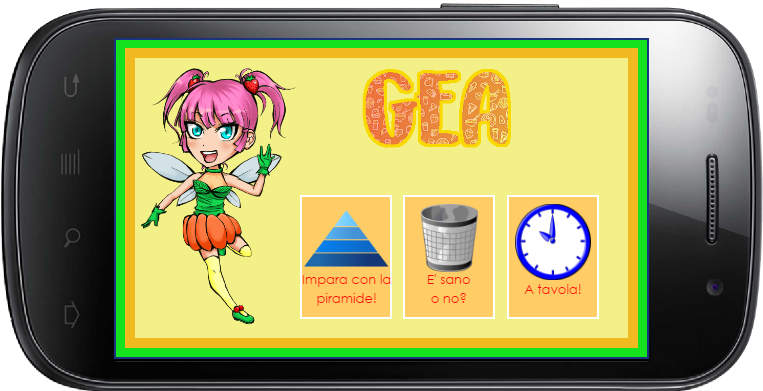
\includegraphics[width=\textwidth]{Images/Mockup/schermatainiziale}
\caption{Schermata iniziale mockup}
\label{fig:Schermata iniziale}
\end{figure}
\clearpage
\subsubsection{Scelta livello difficoltà}
Il mockup in Figura \ref{fig:Scelta livello difficoltà} mostra la schermata per la scelta del livello di difficoltà che si presenta dopo avere selezionato qualsiasi dei tre giochi. Qui, in base alla preparazione del bambino, la terapista può decidere se la difficoltà presentata sia di livello "Facile", "Medio" o "Difficile". Vi è inoltre la presenza del tasto "Indietro" per dare la possibilità di tornare alla schermata principale nel caso in cui sia stato selezionato il gioco errato e si voglia compiere nuovamente la scelta. 

\vspace{70pt}

\begin{figure}[htbp]
\centering
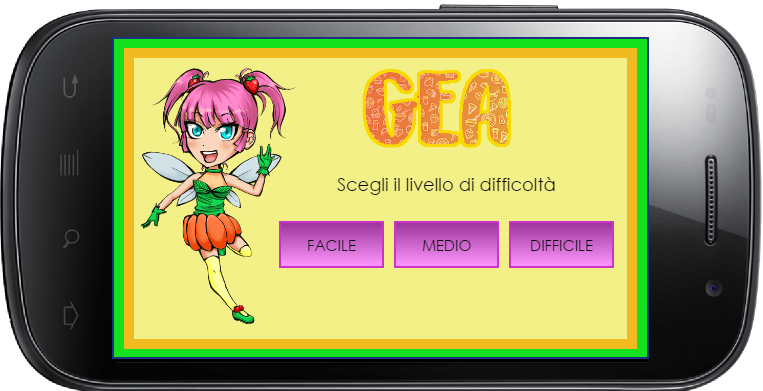
\includegraphics[width=\textwidth]{Images/Mockup/livelli}
\caption{Scelta livello difficoltà mockup}
\label{fig:Scelta livello difficoltà}
\end{figure}
\clearpage
\subsubsection{Primo gioco: Impara con la piramide}
Il mockup in Figura \ref{fig:Impara con la piramide} mostra la schermata che comparirà dopo aver scelto di giocare a "Impara con la piramide" e dopo aver selezionato il livello di difficoltà desiderato. La schermata che appare spiega molto brevemente quello che il bambino dovrà fare giocando e quindi l'obiettivo da raggiungere.
\vspace{70pt}
\begin{figure}[htbp]
\centering
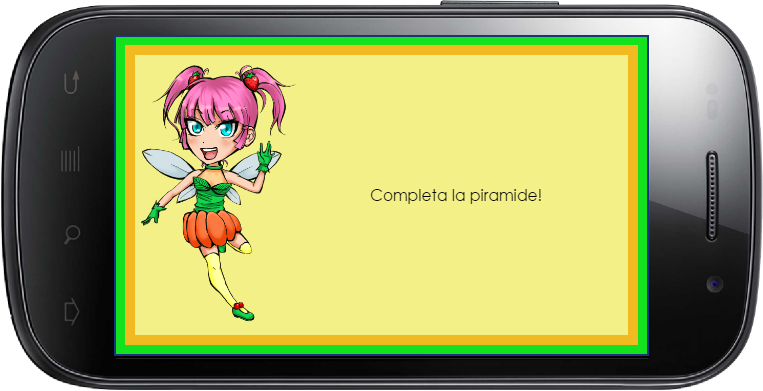
\includegraphics[width=\textwidth]{Images/Mockup/gioco1}
\caption{Impara con la piramide mockup}
\label{fig:Impara con la piramide}
\end{figure}
\clearpage

Il mockup in Figura \ref{fig:Piramide} mostra la schermata successiva a quella esplicativa per quanto riguarda il gioco "Impara con la piramide". Qui viene mostrata al bambino l'intera piramide alimentare che il bambino dovrà via via completare durante il gioco.
\vspace{70pt}
\begin{figure}[htbp]
\centering
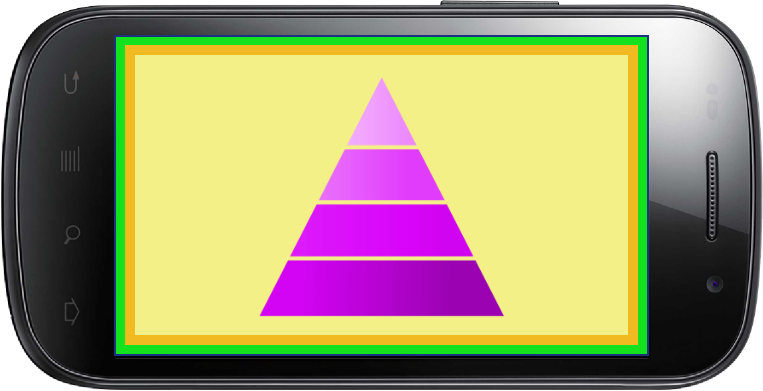
\includegraphics[width=\textwidth]{Images/Mockup/piramide}
\caption{Piramide mockup}
\label{fig:Piramide}
\end{figure}
\clearpage

Il mockup in Figura \ref{fig:Piramide proseguimento} viene presentata dopo aver mostrato l'intera piramide. Qui ci si focalizza su un preciso livello della piramide alimentare che deve essere completato e si mostrano al bambino due alimenti tra cui dover scegliere per effettuare il corretto completamento.
\vspace{70pt}
\begin{figure}[htbp]
\centering
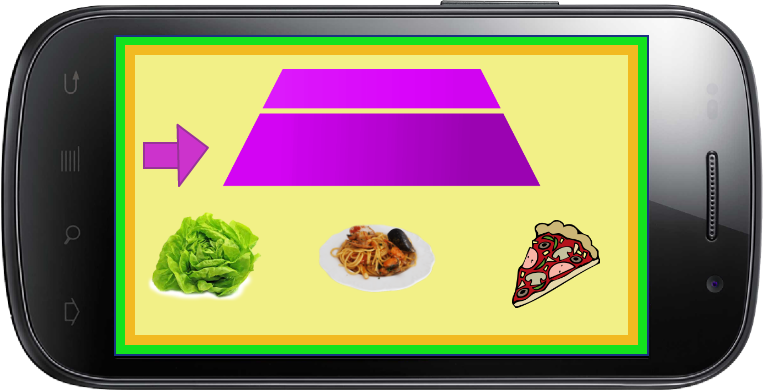
\includegraphics[width=\textwidth]{Images/Mockup/piramide2}
\caption{Piramide proseguimento mockup}
\label{fig:Piramide proseguimento}
\end{figure}
\clearpage

\subsubsection{Secondo gioco: E' sano o no?}
Il mockup in Figura \ref{fig:E' sano o no?} mostra la schermata che comparirà dopo aver scelto di giocare a "E' sano o no?" e dopo aver selezionato il livello di difficoltà desiderato. La schermata che appare spiega molto brevemente quello che il bambino dovrà fare giocando e quindi l'obiettivo da raggiungere.
\vspace{70pt}
\begin{figure}[htbp]
\centering
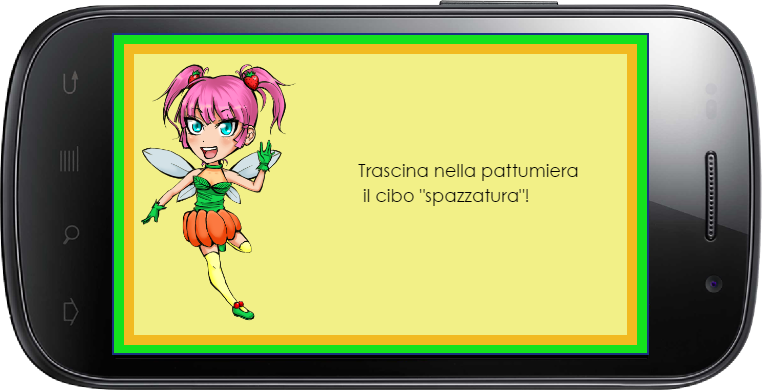
\includegraphics[width=\textwidth]{Images/Mockup/gioco2}
\caption{E' sano o no? mockup}
\label{fig:E' sano o no?}
\end{figure}
\clearpage

Il mockup in Figura \ref{fig:Schermata "E' sano o no?"} mostra la schermata successiva a quella esplicativa per quanto riguarda il gioco "E' sano o no?". Qui vengono mostrati al bambino due pietanze tra le quali deve scegliere il cibo "spazzatura" e "buttarlo" con lo sguardo nella pattumiera presente sulla destra della schermata.
\vspace{70pt}
\begin{figure}[htbp]
\centering
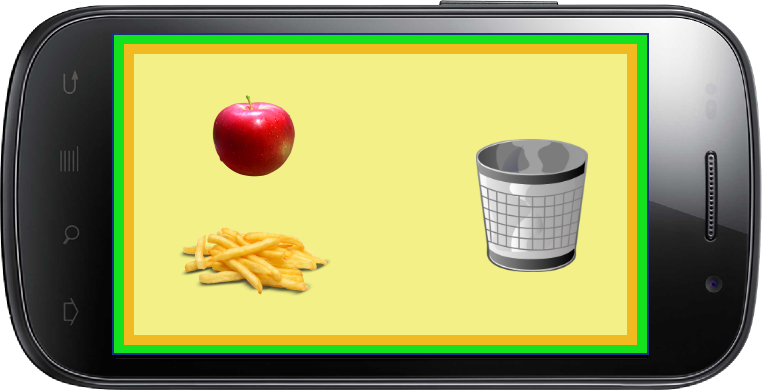
\includegraphics[width=\textwidth]{Images/Mockup/sano}
\caption{Schermata "E' sano o no?" mockup}
\label{fig:Schermata "E' sano o no?"}
\end{figure}
\clearpage

Il mockup in Figura \ref{fig:Scelta "E' sano o no?"} mostra la schermata relativa al compimento di una scelta: nel caso presentato la scelta è errata.
\vspace{70pt}
\begin{figure}[htbp]
\centering
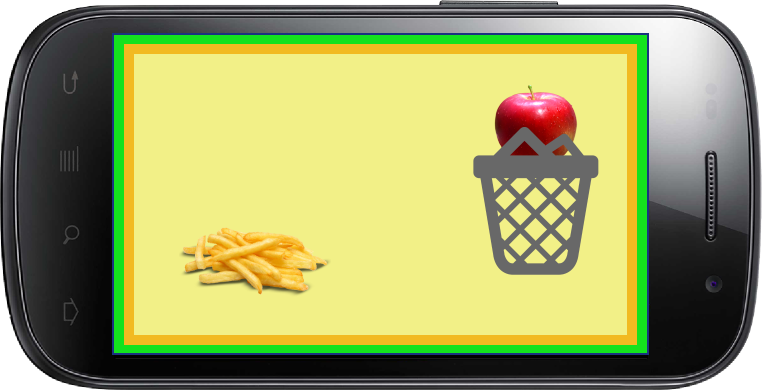
\includegraphics[width=\textwidth]{Images/Mockup/sanoscelta}
\caption{Scelta cibo "spazzatura" mockup}
\label{fig:Scelta "E' sano o no?"}
\end{figure}
\clearpage

Il mockup in Figura \ref{fig:Feedback scelta errata} mostra il feedback per quanto riguarda una scelta erronea: compare il volto della mascotte con espressione rattristata e scritta esplicativa di risposta errata.
\vspace{70pt}
\begin{figure}[htbp]
\centering
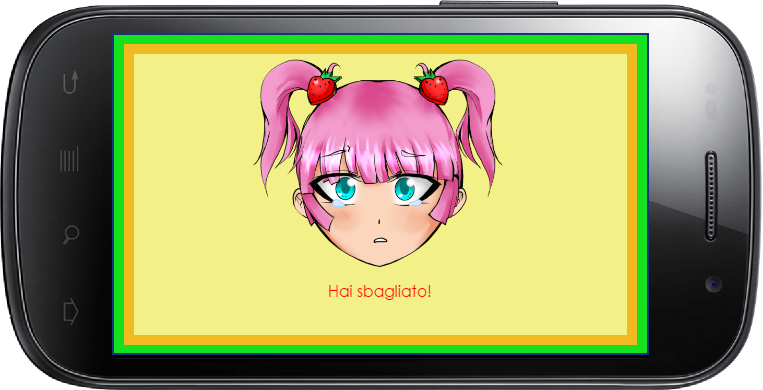
\includegraphics[width=\textwidth]{Images/Mockup/sanofeedback}
\caption{Feedback scelta errata mockup}
\label{fig:Feedback scelta errata}
\end{figure}
\clearpage


\subsubsection{Terzo gioco: A tavola!}
Il mockup in Figura \ref{fig:A tavola!} mostra la schermata che comparirà dopo aver scelto di giocare a "A tavola!" e dopo aver selezionato il livello di difficoltà desiderato. La schermata che appare spiega molto brevemente quello che il bambino dovrà fare giocando e quindi l'obiettivo da raggiungere.
\vspace{70pt}
\begin{figure}[htbp]
\centering
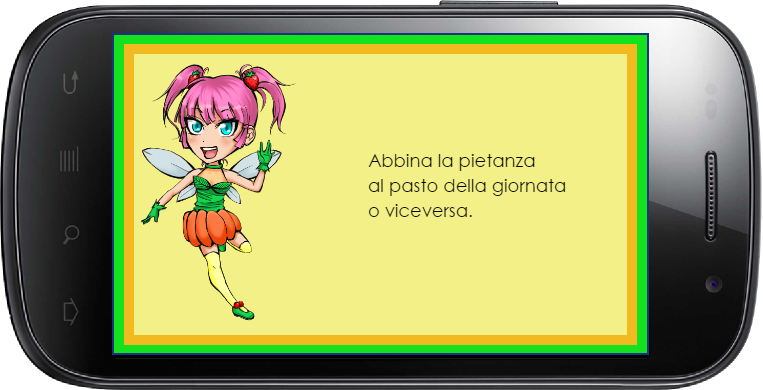
\includegraphics[width=\textwidth]{Images/Mockup/gioco3}
\caption{A tavola! mockup}
\label{fig:A tavola!}
\end{figure}
\clearpage

Il mockup in Figura \ref{fig:Schermata "A tavola!"} mostra la schermata successiva a quella esplicativa per quanto riguarda il gioco "A tavola!". Qui vengono mostrati al bambino una pietanza e due possibili pasti del giorno: egli deve scegliere qual è il pasto più adatto per consumare quella pietanza. Il gioco si può presentare anche nella forma opposta ossia scegliere fra due piatti quale sia più adatto per il pasto indicato.
\vspace{70pt}
\begin{figure}[htbp]
\centering
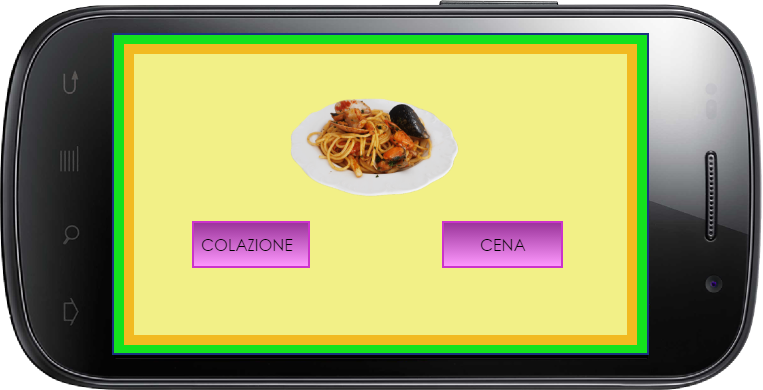
\includegraphics[width=\textwidth]{Images/Mockup/atavola}
\caption{Schermata "A tavola!" mockup}
\label{fig:Schermata "A tavola!"}
\end{figure}
\clearpage

Il mockup in Figura \ref{fig:Scelta "A tavola!"} mostra la schermata relativa al compimento di una scelta: nel caso presentato la scelta è corretta.
\vspace{70pt}
\begin{figure}[htbp]
\centering
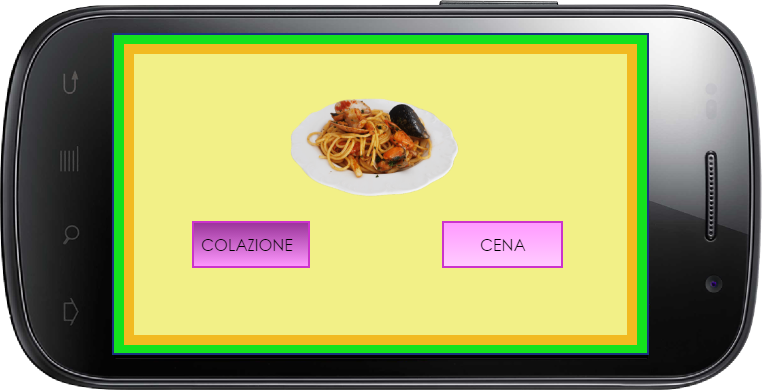
\includegraphics[width=\textwidth]{Images/Mockup/atavolascelta}
\caption{Scelta pasto mockup}
\label{fig:Scelta "A tavola!"}
\end{figure}
\clearpage

Il mockup in Figura \ref{fig:Feedback scelta corretta} mostra il feedback per quanto riguarda una scelta corretta: compare il volto della mascotte con espressione sorridente e scritta esplicativa di risposta esatta.
\vspace{70pt}
\begin{figure}[htbp]
\centering
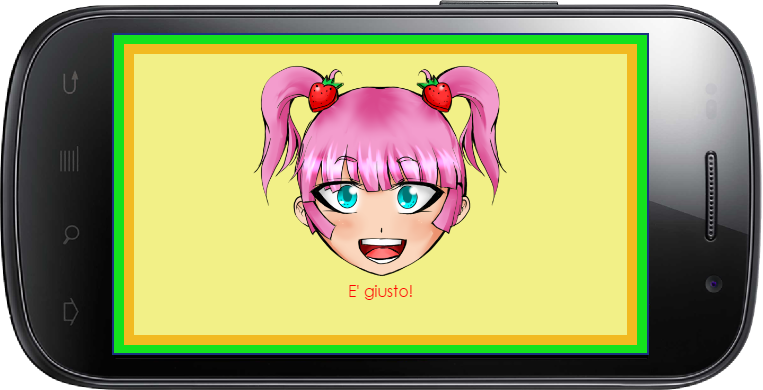
\includegraphics[width=\textwidth]{Images/Mockup/atavolafeedback}
\caption{Feedback scelta corretta mockup}
\label{fig:Feedback scelta corretta}
\end{figure}
\clearpage
\newpage
\section{Implementazione} \label{sec:tecn}

\subsection{Architettura hardware} \label{subsec:hard}
I terapisti hanno bisogno di poter vedere quello che il bambino compie durante l'esperienza di gioco per cui abbiamo la necessità di replicare lo schermo dello smartphone su pc: questo verrà effettuato con l'uso di Google Chromecast.
\vspace{70pt}
\begin{figure}[htbp]
\centering
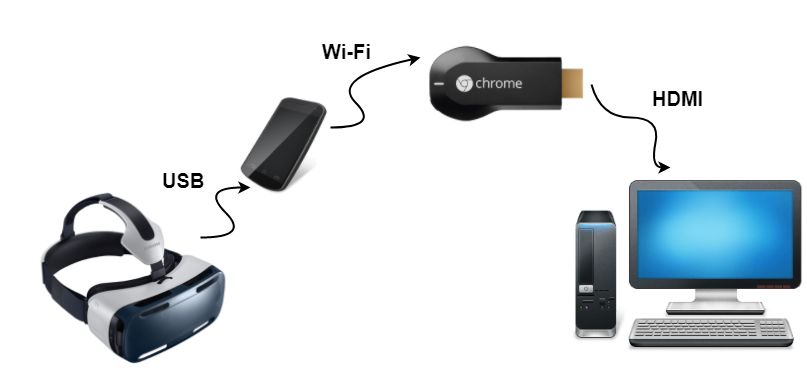
\includegraphics[width=\textwidth]{Images/hardware}
\caption{Architettura hardware}
\label{fig:hardware}
\end{figure}
\clearpage

\subsection{Architettura software} \label{subsec:soft}
L'architettura software prevede la comunicazione di tre moduli principali: l'applicazione \acs{gea}, con cui il terapista (nella scelta iniziale del livello di difficoltà) comunica, che è collegata al programma di gestione di orientamento visivo (necessario per captare i movimenti e il focus del bambino) del \acs{vr} e che trasferisce i dati al \acs{pc} del terapista che può quindi monitorare l'avanzamento del gioco e dare perciò eventuali suggerimenti al paziente.
\vspace{70pt}
\begin{figure}[htbp]
\centering
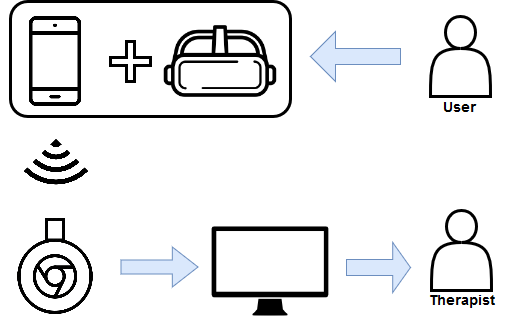
\includegraphics[width=\textwidth]{Images/software}
\caption{Architettura software}
\label{fig:software}
\end{figure}
\clearpage

\subsection{Linguaggi di programmazione e software utilizzati} \label{subsec:ling}
Di seguito vengono elencati i linguaggi di programmazione e i software utilizzati per sviluppare l'applicazione in realtà virtuale \acs{gea}.
\subsubsection{Linguaggi di programmazione}
\begin{itemize}
	\item \acs{html}
	\item \acs{css}
	\item JavaScript
	\item A-Frame
	\item \acs{php}
	\item JQuery
\end{itemize}
\subsubsection{Software}
\begin{itemize}
	\item Brackets
	\item AlterVista
	\item FileZilla
	\item Imgur
\end{itemize}
\newpage
\section{Valutazione} \label{sec:val}
\newpage
\section{Documentazione Tecnica} \label{sec:tecdoc}
\newpage
\section{Appendice} \label{sec:app}

\subsection{Tool utilizzati} \label{subsec:tool}

\begin{itemize}
	\item \LaTeX\ e l'editor TeXMaker : per redigere e strutturare questo documento
	\item Pencil : per la creazione dei mockups
\end{itemize}

\subsection{Acronimi} \label{acr}
Di seguito la lista degli acronimi utilizzati all'interno del documento:

%------------Acronyms----------
\begin{acronym}[NDD] %put here the first acronym

\acro{ndd}[NDD]{NeuroDevelopmental Disorder}
\acro{asd}[ASD]{Autistic Spectrum Disorders}
\acro{adhd}[ADHD]{Attention Deficit Hyperactivity Disorder}
\acro{gea}[GEA]{Gioco Educazione Alimentare}
\acro{vr}[VR]{Virtual Reality}
\acro{usb}[USB]{Universal Serial Bus}
\acro{hdmi}[HDMI]{High-Definition Multimedia Interface}
\acro{pc}[PC]{Personal Computer}
\acro{html}[HTML]{HyperText Markup Language}
\acro{css}[CSS]{Cascading Style Sheets}
\acro{php}[PHP]{Hypertext Preprocessor}

%lists of used acronyms

\end{acronym}

\subsection{Bibliografia} \label{subsec:biblio}

%----------------------------------------------------------------------------------------
%\newpage
%\pagestyle{empty}
%\bibliographystyle{unsrt}
%\bibliography{sample}
%----------------------------------------------------------------------------------------

\end{document}